% !TeX TXS-program:compile = txs:///pdflatex/[--shell-escape]
\documentclass[handout, aspectratio=169, 10pt]{beamer}

% packages
\usepackage{newpxmath} % math font is Palatino compatible
% \usepackage[nomath]{fontspec}

\usepackage{setspace}
\usepackage{xcolor}
\usepackage{soul} % for \st
\usepackage{hyperref} % for links
\definecolor{links}{HTML}{2A1B81}
\hypersetup{colorlinks,linkcolor=,urlcolor=links}


% table stuff
\usepackage{chronosys}
\usepackage{verbatim}
% \pagenumbering{arabic}
\usepackage{tabularx}
\usepackage{booktabs}
\usepackage{ragged2e}
\usepackage{mathtools}

% R Code
\usepackage{listings}
\usepackage{courier}
\lstset{basicstyle=\scriptsize\ttfamily,breaklines=true}
\lstset{framextopmargin=50pt,frame=bottomline}

% themes
\usetheme[progressbar=frametitle, block=fill]{metropolis}
\useoutertheme{metropolis}
\useinnertheme{metropolis}

% colors
\definecolor{dimwhite}{rgb}{0.99, 0.99, 0.99}
\definecolor{charcoal}{rgb}{0.21, 0.27, 0.31}
\definecolor{slategray}{rgb}{0.44, 0.5, 0.56}
\definecolor{dimgray}{rgb}{0.41, 0.41, 0.41}
\definecolor{bleudefrance}{rgb}{0.19, 0.55, 0.91}

% beamer options
\setbeamercolor{author}{fg=charcoal}
\setbeamercolor{background canvas}{bg=white}
\setbeamercolor{section in toc}{fg=charcoal}
\setbeamercolor{subsection in toc}{fg=dimgray}
\setbeamercolor{frametitle}{bg=dimwhite, fg=charcoal}
\setbeamercolor{progress bar}{fg=slategray, bg=fg!50!black!30}
\setbeamercovered{transparent}
\setbeamertemplate{itemize items}[triangle]
\setbeamertemplate{itemize subitem}[circle]
\setbeamertemplate{itemize subsubitem}[square]
\setbeamersize{text margin left=7mm,text margin right=7mm} 

% new commands
\newcommand{\q}[1]{``#1''}
\newcommand{\hs}[1]{\textsc{\hfill\scriptsize\color{dimgray}#1}}
\newcommand{\g}[1]{{\color{gray}#1}}
\newcommand{\dg}[1]{{\color{dimgray}#1}}
\newcommand{\sg}[1]{{\color{slategray}#1}}
\newcommand{\bdf}[1]{{\color{bleudefrance}#1}}
\newcommand{\itemcolor}[1]{\renewcommand{\makelabel}[1]{\color{#1}\hfil ##1}}
\newcommand\Wider[2][2em]{
\makebox[\linewidth][c]{
  \begin{minipage}{\dimexpr\textwidth+#1\relax}
  \raggedright#2
  \end{minipage}
  }
}

% misc
\linespread{1.35}

% minted (risky)
\usepackage[cache=false]{minted}

% Math stuff
\newcommand{\norm}[1]{\left\lVert#1\right\rVert}
\newcommand{\R}{\mathbb{R}}
\newcommand{\E}{\mathbb{E}}
\newcommand{\V}{\mathbb{V}}
\newcommand{\probP}{\text{I\kern-0.15em P}}
\newcommand{\ol}{\overline}
%\newcommand{\ul}{\underline}
\newcommand{\pp}{{\prime \prime}}
\newcommand{\ppp}{{\prime \prime \prime}}
\newcommand{\policy}{\gamma}
\newcommand{\plim}{ \overset{p}{\to}}
\newcommand{\hnot}{ \overset{H_0}{\to}}

% Causal Graphs
\usetikzlibrary{shapes,decorations,arrows,calc,arrows.meta,fit,positioning}
\tikzset{
    -Latex,auto,node distance =1 cm and 1 cm,semithick,
    state/.style ={ellipse, draw, minimum width = 0.7 cm},
    point/.style = {circle, draw, inner sep=0.04cm,fill,node contents={}},
    bidirected/.style={Latex-Latex,dashed},
    el/.style = {inner sep=2pt, align=left, sloped}
}

\setbeamersize{text margin left=10pt,text margin right=10pt}


\begin{document}


\title[L5-Wage Equation Example]{ Econometrics I}
\subtitle{Lecture 5: Extended Example: The Wage Equation}
\author{Chris Conlon}
\date{Fall 2025}
\maketitle






\begin{frame}{Mincerian Regression}
\begin{itemize}
	\item Recall the Mincerian regression (wage equation):\[
	\ln wage_i = \beta_0 + \beta_{ed} Education_i + \beta_{exp} Experience_i + \beta_{Fem} Female_i + \dots + \varepsilon_i
	\]

	\smallskip
	\item Let's revisit estimating this with the Cornwell and Rupert (NLSY) data. 
\end{itemize}
\end{frame}




\begin{frame}{Process the data}
\begin{center}
	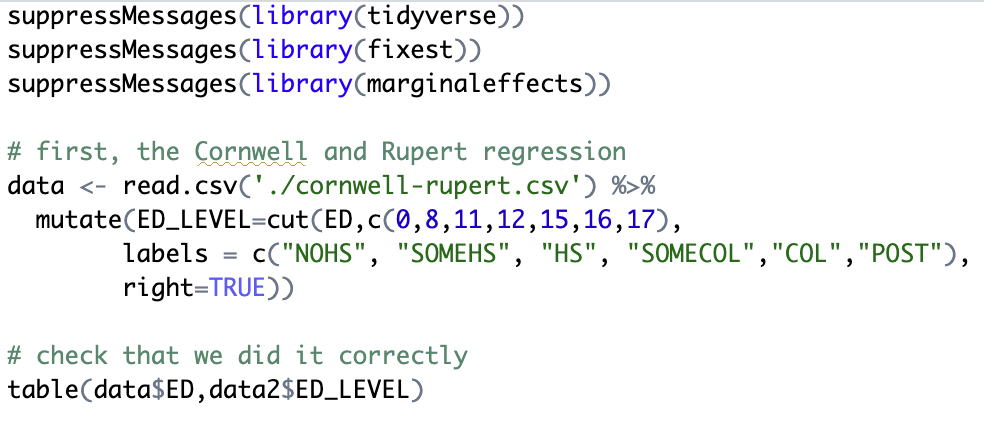
\includegraphics [width=.9\textwidth]{code_0}\\
\end{center}
\end{frame}



\begin{frame}{Interpreting $\widehat{\beta}$}
\begin{columns}
\begin{column}{0.5\textwidth}
\begin{figure}
\flushleft
	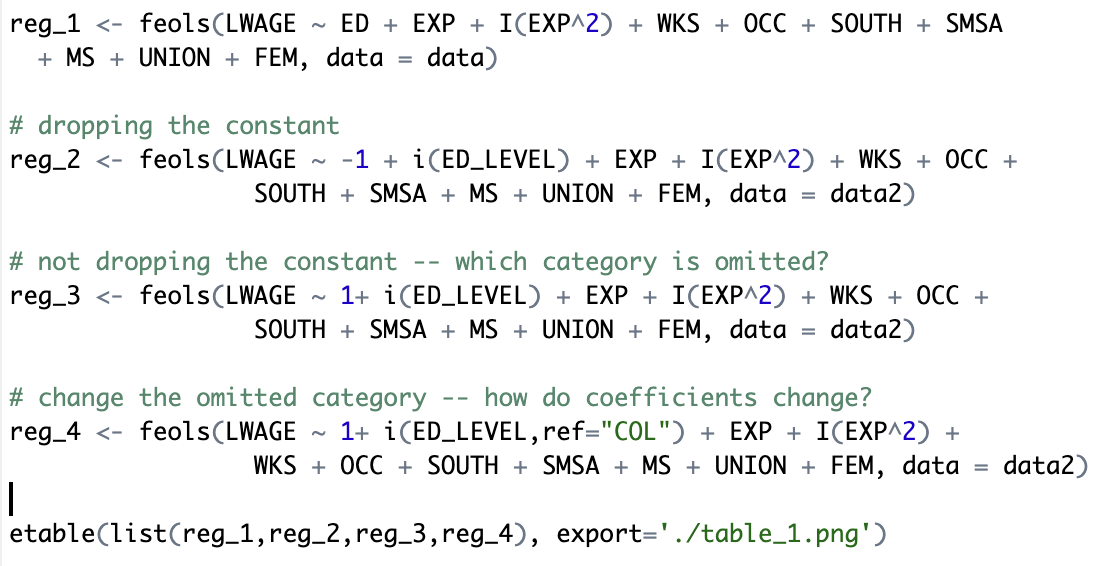
\includegraphics [width=\textwidth]	{code_1}
\end{figure}
\small
\only<1>{
	Notice I've used the $\texttt{i}(\cdot)$ command to make categorical variables into dummies and $\texttt{I}(\cdot)$ to do polynomial terms.
}
\only<2>{
	Note on interpreting effects with $\log(y_i)\approx 1+\beta$:
\begin{itemize}
	\item $\exp \left( -.3892\right) = .6826$
		\item $\exp \left( .05654\right) = 1.057$
\end{itemize}
}
\only<3>{
	\begin{itemize}
	\item In Regression \#1, what does the coeffcient $\beta_{ED}$ mean?
	\item What about in Regression \#2? What is the interpretation of $\beta_{somecol}$?
	\item How about in Regression \#3? and \#4?
\end{itemize}
}
\end{column}
\begin{column}{0.5\textwidth}
\begin{figure}
\flushleft
	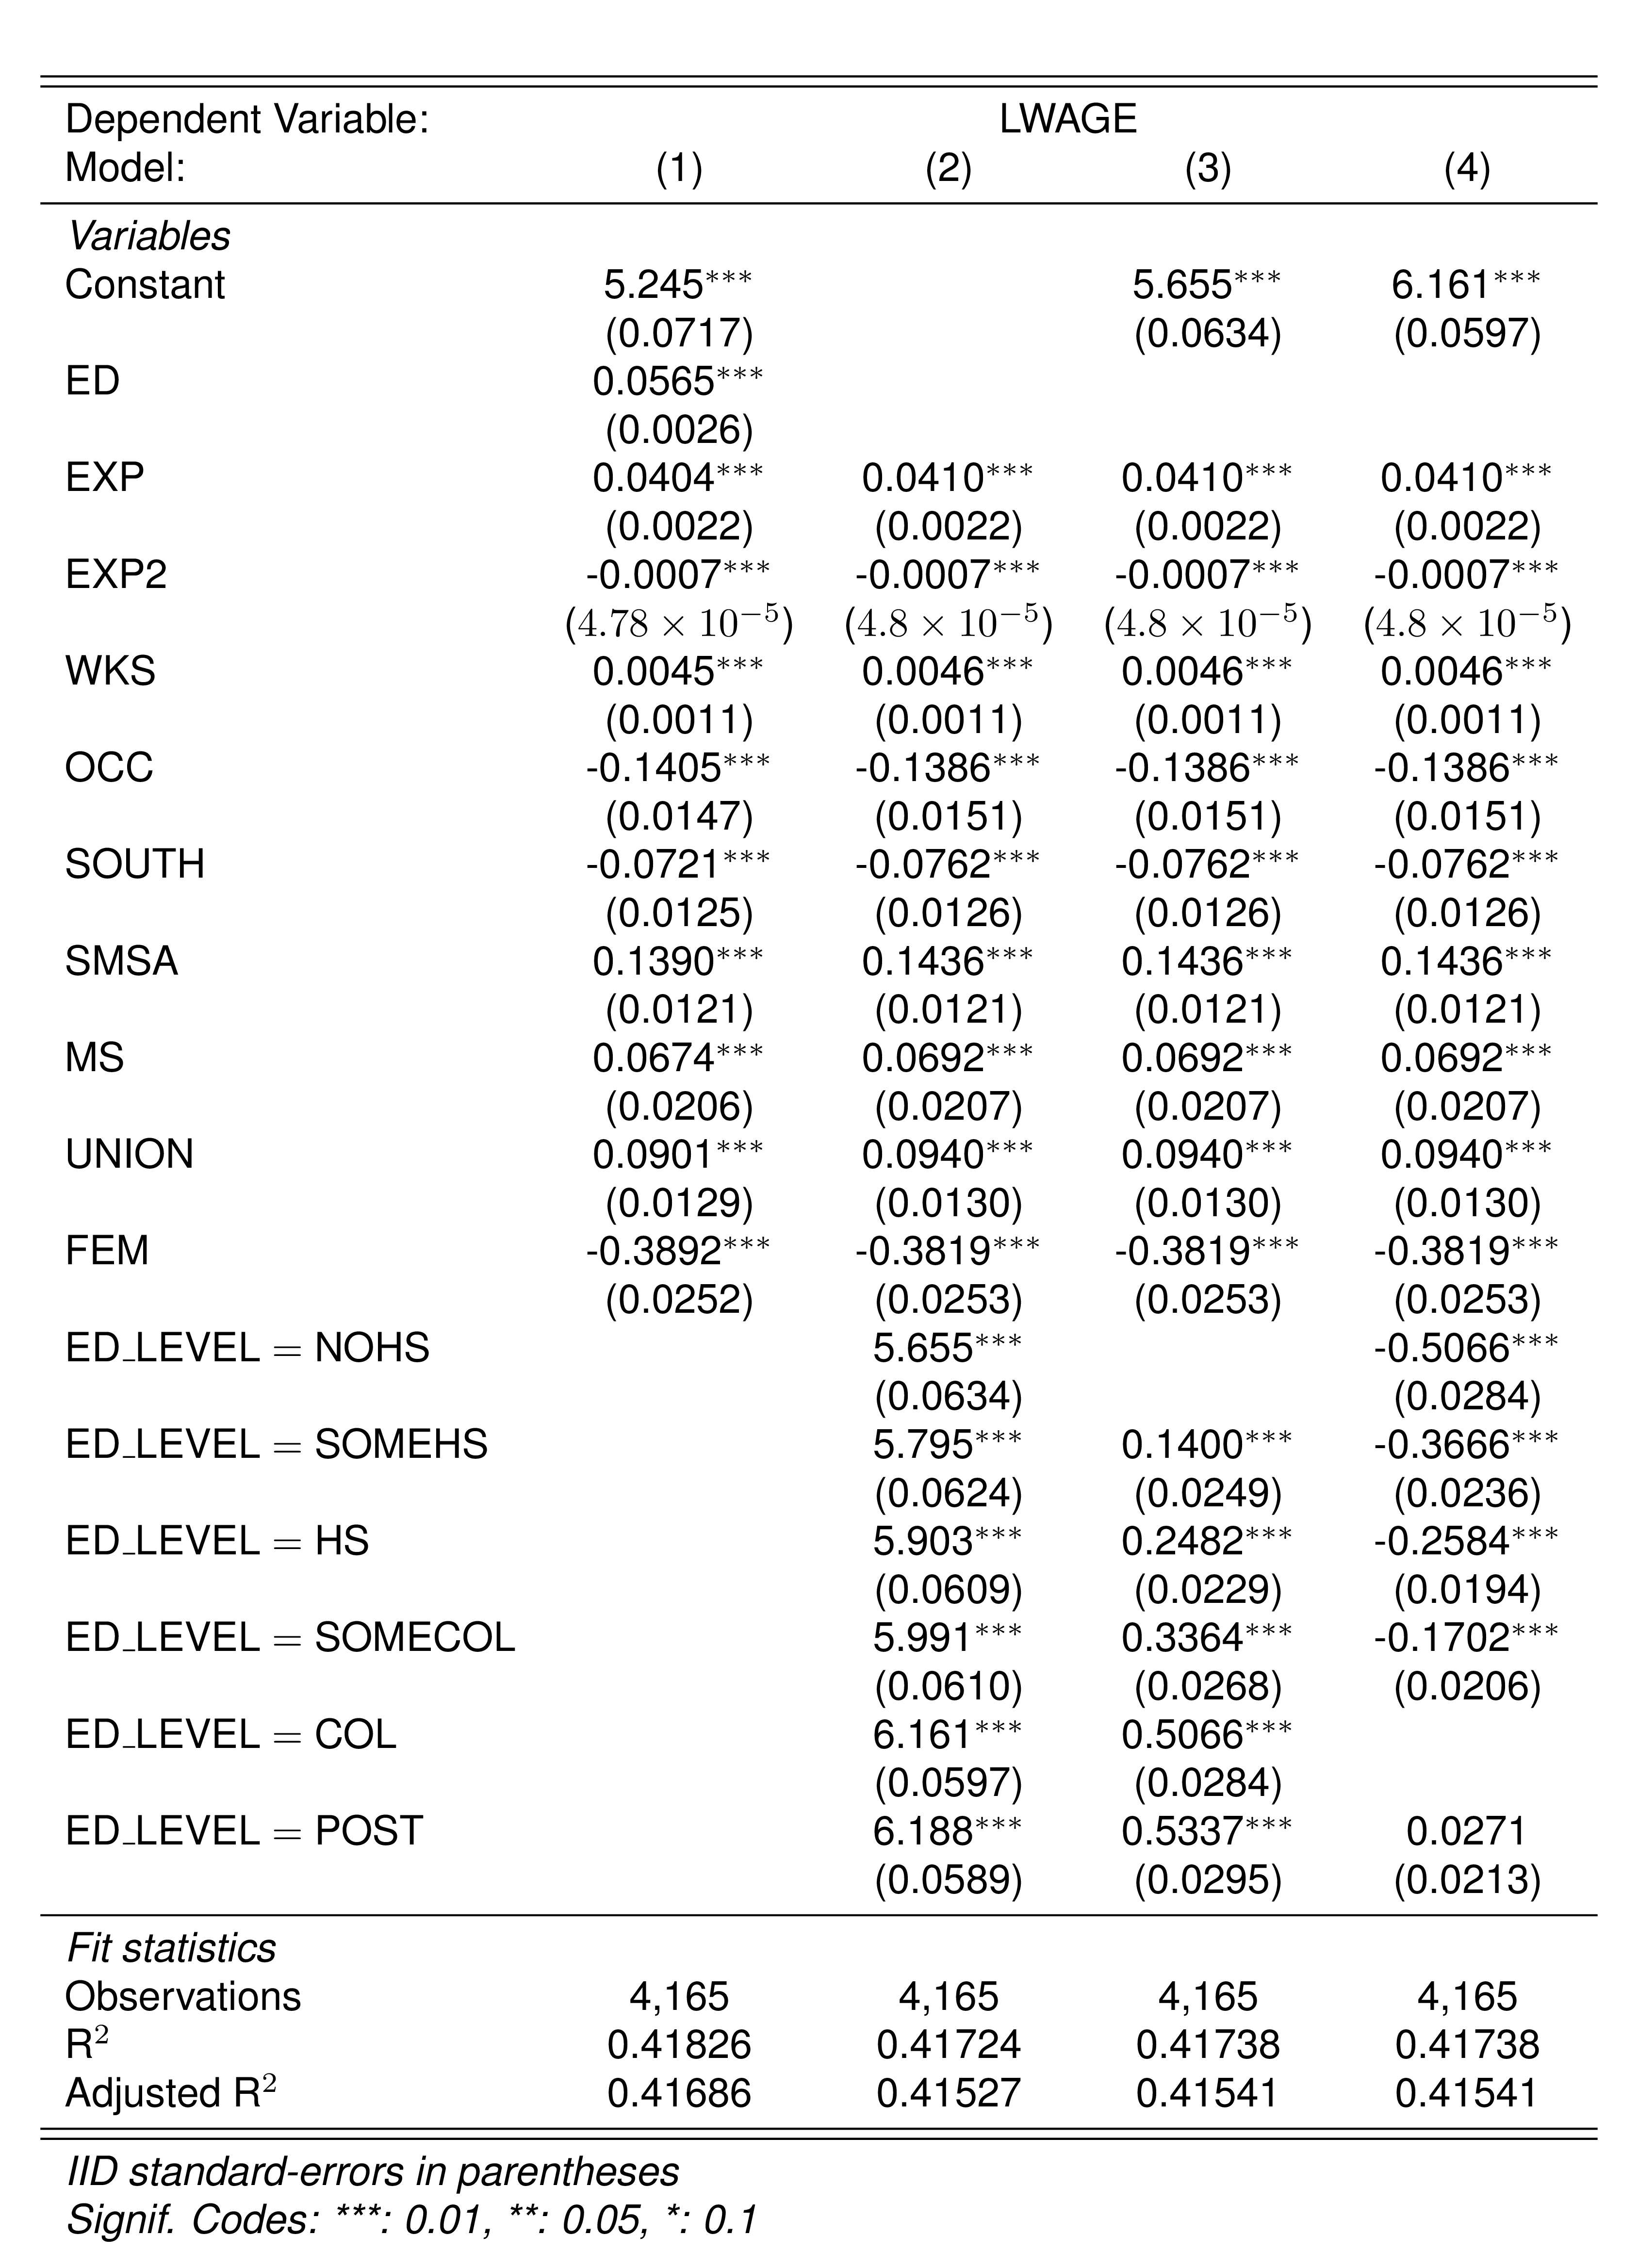
\includegraphics [width=0.8\textwidth]	{table_1}
\end{figure}
\end{column}
\end{columns}	
\end{frame}



\begin{frame}{Formulating Linear Hypotheses}
\begin{columns}
\begin{column}{0.5\textwidth}
\begin{figure}
\flushleft
	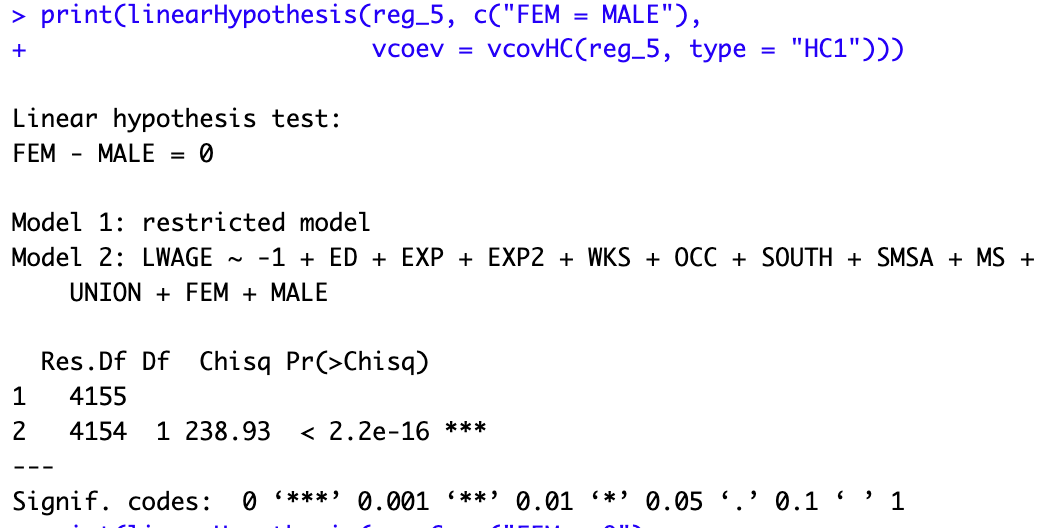
\includegraphics [width=\textwidth]	{hypothesis_1}
\end{figure}

\end{column}
\begin{column}{0.5\textwidth}
\begin{figure}
\flushleft
	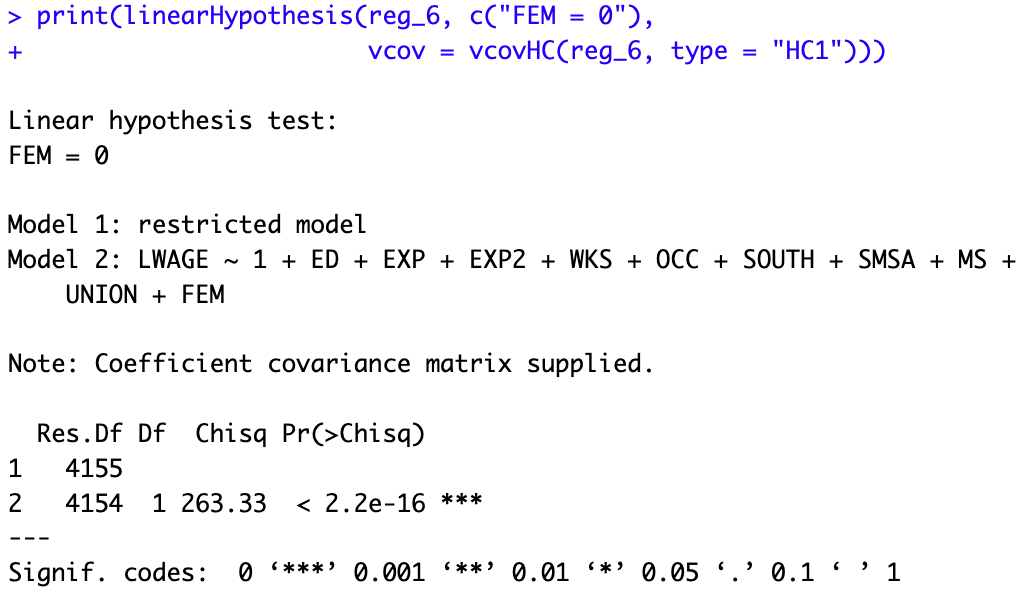
\includegraphics [width=\textwidth]	{hypothesis_2}
\end{figure}
\end{column}
\end{columns}
We can test the same hypothesis with an $F$-test two different ways:
\begin{itemize}
	\item $H_0: \beta_{M} = \beta_{F}$ if we omit the constant.
	\item $H_0: \beta_{F}=0$ if we include the constant.
\end{itemize}
\end{frame}



\begin{frame}{Correlation in F-Tests}
\begin{columns}
\begin{column}{0.5\textwidth}
\begin{figure}
\flushleft
	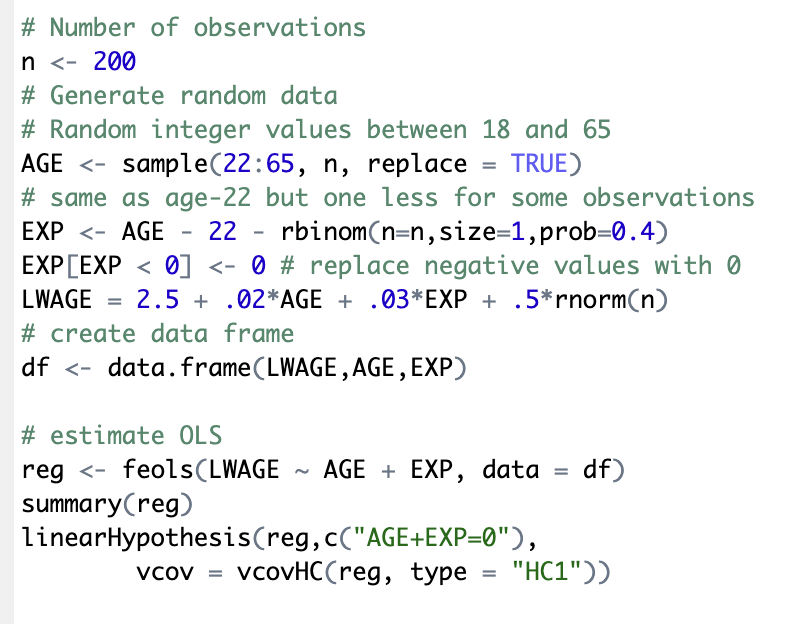
\includegraphics [width=\textwidth]	{correlation_code}
\end{figure}

\end{column}
\begin{column}{0.5\textwidth}
\begin{figure}
\flushleft
	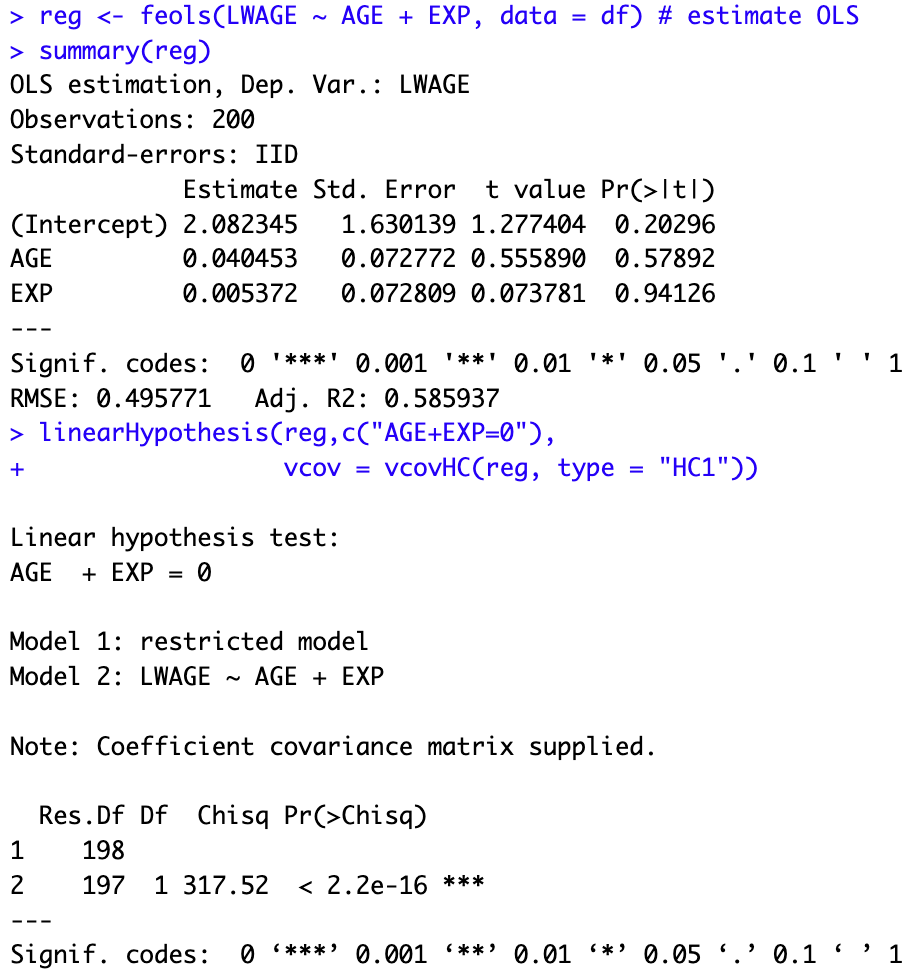
\includegraphics [width=0.8\textwidth]	{correlation_test}
\end{figure}
\end{column}
\end{columns}
Notice that $t$-stats are not significant but $F$-test is huge, why?
\end{frame}



\begin{frame}{Marginal Effects}
Our regression specification contained both linear terms and quadratic terms for experience
\begin{align*}
\ln wage_i = \beta_0 + \beta_{exp} Experience_i + \beta_{exp^2} Experience^2_i + \beta X_i + \varepsilon_i
\end{align*}
We can compute the marginal effect of an additional year of experience as:
\begin{align*}
\frac{\partial \ln wage_i}{\partial Experience_i} = \beta_{exp} + 2 \beta_{exp^2} Experience_i \equiv g(\boldsymbol{\beta}).
\end{align*}
\begin{itemize}
\item Note: We cannot simply interpret $\beta_{exp}$ or $\beta_{exp^2}$ on their own.
\item To compute standard errors on marginal effects, we can't just look at the $t$-stats.
\item This is also an issue in \alert{nonlinear models} like Probit and Logit (later).
\end{itemize}
\end{frame}


\begin{frame}{Delta Method II}
	\small
\begin{itemize}
\item Suppose we have an asymptotic distribution for an estimator: 
\[
\sqrt{n}\left(\boldsymbol{b}-\boldsymbol{\beta}\right)\Rightarrow_{d}\mathcal{N}\left(\boldsymbol{0},\boldsymbol{\Sigma}\right).
\]
\item Then the asymptotic distribution of a function of the estimator is
\[
\sqrt{n}\left(g\left(\boldsymbol{b}\right)-g\left(\boldsymbol{\beta}\right)\right)\Rightarrow_{d}\mathcal{N}\left(\boldsymbol{0},\left(\nabla g\left(\boldsymbol{\beta}\right)\right)'\boldsymbol{\Sigma}\nabla g\left(\boldsymbol{\beta}\right)\right),
\]
where $\nabla g\left(\boldsymbol{\beta}\right)$ is the gradient of
$g\left(\boldsymbol{\beta}\right)$: 
\[
\nabla g\left(\boldsymbol{\beta}\right)=\left(\begin{array}{c}
\frac{\partial g\left(\boldsymbol{\beta}\right)}{\partial\beta_{1}},
\frac{\partial g\left(\boldsymbol{\beta}\right)}{\partial\beta_{2}},
\cdots,
\frac{\partial g\left(\boldsymbol{\beta}\right)}{\partial\beta_{K}}
\end{array}\right)^T.
\]
\item Note that we can estimate $\nabla g\left(\boldsymbol{\beta}\right)$
with $\nabla g\left(\boldsymbol{b}\right)$.
\item Notice how the covariance between the coefficients $\boldsymbol{\Sigma}$ matters!
\item What is the expression for the standard error of the marginal effect of experience?
\end{itemize}
\end{frame}



\begin{frame}{Delta Method / Marginal Effects in R}
\begin{columns}
\begin{column}{0.5\textwidth}
\begin{figure}
\flushleft
	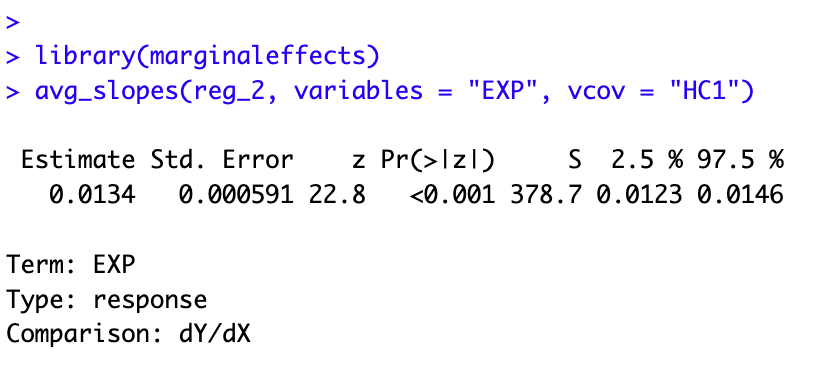
\includegraphics [width=0.8\textwidth]	{marginal_effects}
\end{figure}
Here we get the answer \alert{correct}
\end{column}
\begin{column}{0.5\textwidth}
\begin{figure}
\flushleft
	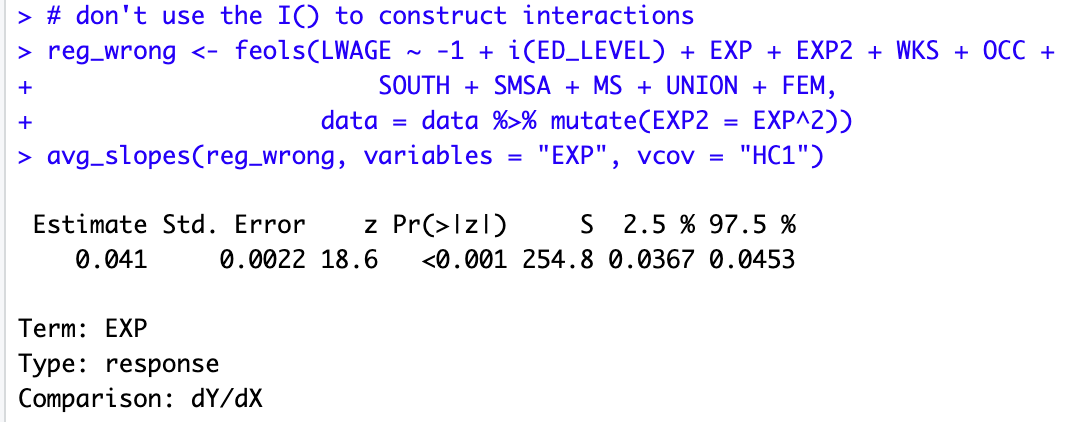
\includegraphics [width=\textwidth]	{marginal_effects2}
\end{figure}
Here we get the answer \alert{wrong}
\end{column}
\end{columns}
What is the exercise we perform in each case?
\end{frame}

\begin{frame}{Bootstrap/ Simulated Asymptotic Distribution}
\begin{itemize}
\item Given the the asymptotic distribution of a parameter estimate
\[
\boldsymbol{b}\sim_{d}\mathcal{N}\left(\boldsymbol{\beta},\boldsymbol{\Sigma}\right),
\]
we have an estimated density function $\hat{f}$. Let $\hat{f}$ be
the multivariate normal density with mean $\boldsymbol{\beta}$ and
variance $\boldsymbol{\Sigma}$.
\item We can simulate the asymptotic distribution of $g\left(\boldsymbol{b}\right)$
by
\begin{itemize}
\item Simulating draws $\boldsymbol{b}_{m}$ for $m=1,2,\dots M$ from $\hat{f}$
\item Computing $g\left(\boldsymbol{b}_{m}\right)$ for each draw
\item Then $\left(g\left(\boldsymbol{b}_{1}\right),g\left(\boldsymbol{b}_{2}\right),\dots,g\left(\boldsymbol{b}_{M}\right)\right)$
will be a simulated asymptotic distribution for $g\left(\boldsymbol{b}\right)$
\end{itemize}
\item This can be useful when you have code to compute $g\left(\cdot\right)$,
but computing the derivative $g\left(\cdot\right)$ would be difficult.
For example, when $g\left(\cdot\right)$ represents an complex behavioral
(or equilibrium) model.
\item Also if you are too lazy to load \texttt{marginaleffects}
\end{itemize}
\end{frame}



\begin{frame}{Boostrap Marginal Effects in R}
\begin{columns}
\begin{column}{0.5\textwidth}
\begin{figure}
\flushleft
	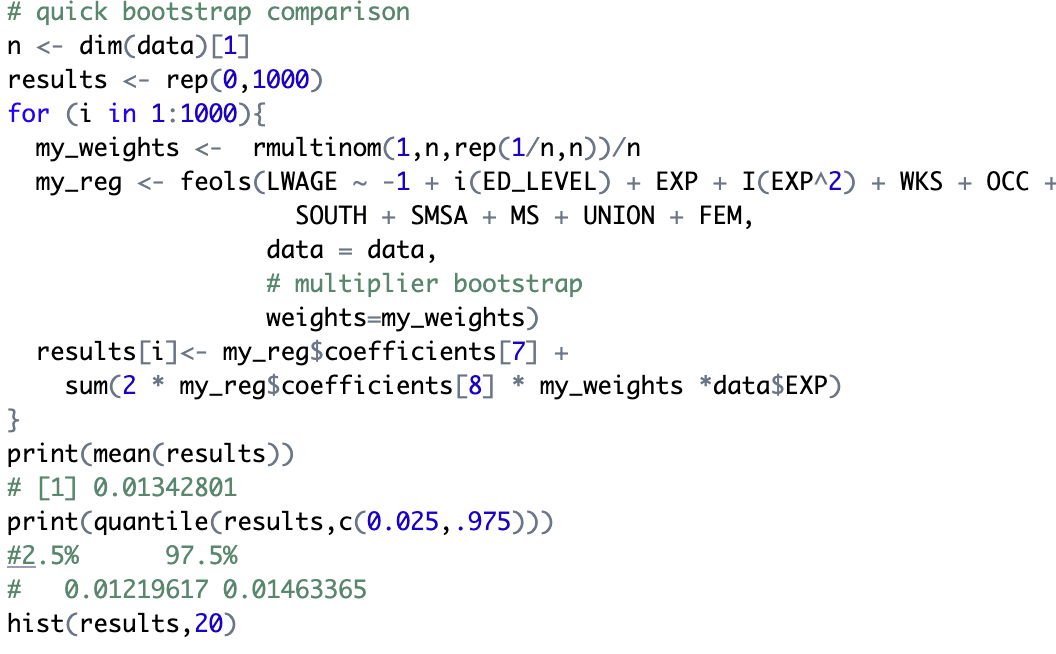
\includegraphics [width=\textwidth]	{boot_code}
\end{figure}
\end{column}
\begin{column}{0.5\textwidth}
\begin{figure}
\flushleft
	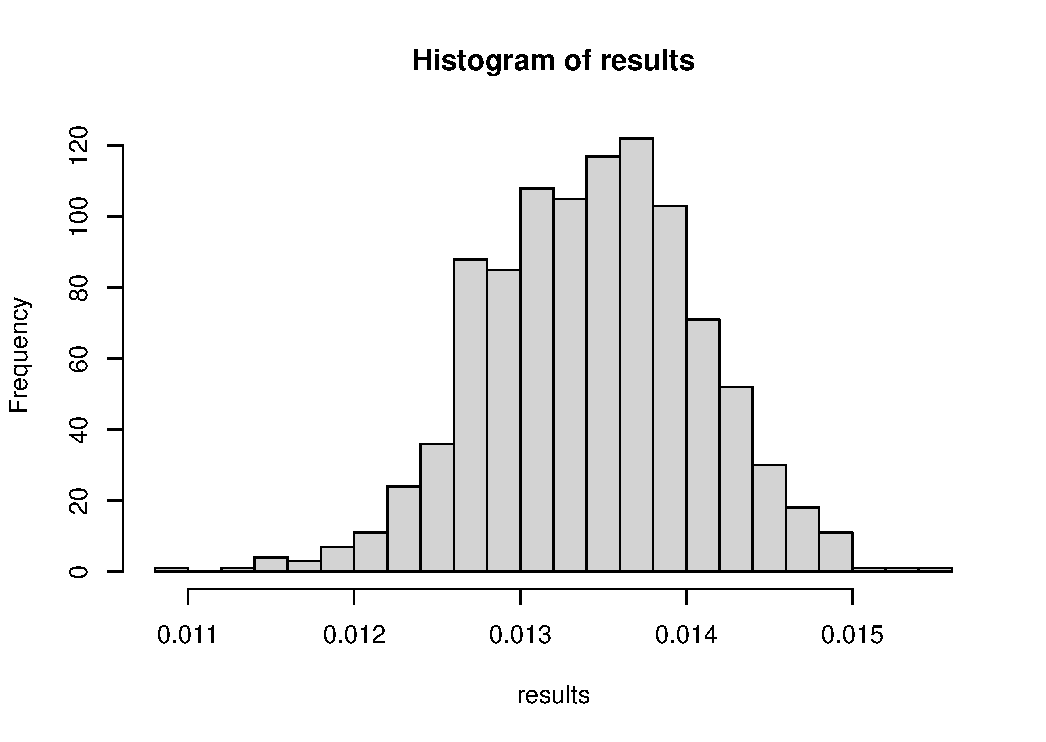
\includegraphics [width=\textwidth]	{boot_plot}\\
\end{figure}
How does the distribution of results compare to delta method? Can we do better?
\end{column}
\end{columns}
\end{frame}



\begin{frame}{Heterogeneous Effects}
	\small
\begin{itemize}
	\item When we have a model of the form \[
		Y_i = \beta_0 + \beta_1 X_{1i} + \varepsilon_i
	\]
	we're implicitly saying that the effect of $X_1$ is the same for all individuals.
	
	\smallskip
	\item Often we would like to relax this, allowing different 
	groups to have different slopes with respect to $X_{1}$.
	
	\smallskip
	\item This is easy as long as the group membership is observed in the data.
	We simply interact the regressor with dummy variables:\[
Y_{i}=\beta_{0}+\beta_{0F}D_{Fi}+\beta_{1}X_{1i}+\beta_{2}X_{1i}D_{Fi}+\varepsilon_{i}
\]
	where $D_{Fi}$ is a dummy variable for whether individual $i$ is female. Note that
	we have allowed for the intercepts and slopes to vary by sex here. 
\item Run this on your own and experiment with $\texttt{i}(\cdot)$ operator and $:$ and $*$.
\end{itemize}
\end{frame}



\begin{frame}{Mincerian Regression: Measurement Error }
\begin{columns}
\begin{column}{0.5\textwidth}
{\small
\begin{itemize}
	\item What happens if one of the variables of interest is measured with error?

	\item Let's say the the recorded education might be one year more or less than the
	person's actual education.

	\item Note: this may already be happening in the data, but let's make it happen more.

\end{itemize}
}
\begin{figure}
\flushleft
	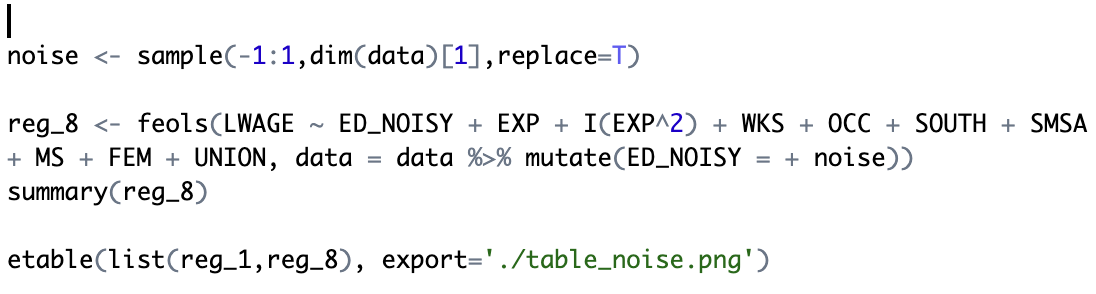
\includegraphics [width=.9\textwidth]	{code_noise}
\end{figure}
\end{column}
\begin{column}{0.5\textwidth}
\begin{figure}
\flushleft
	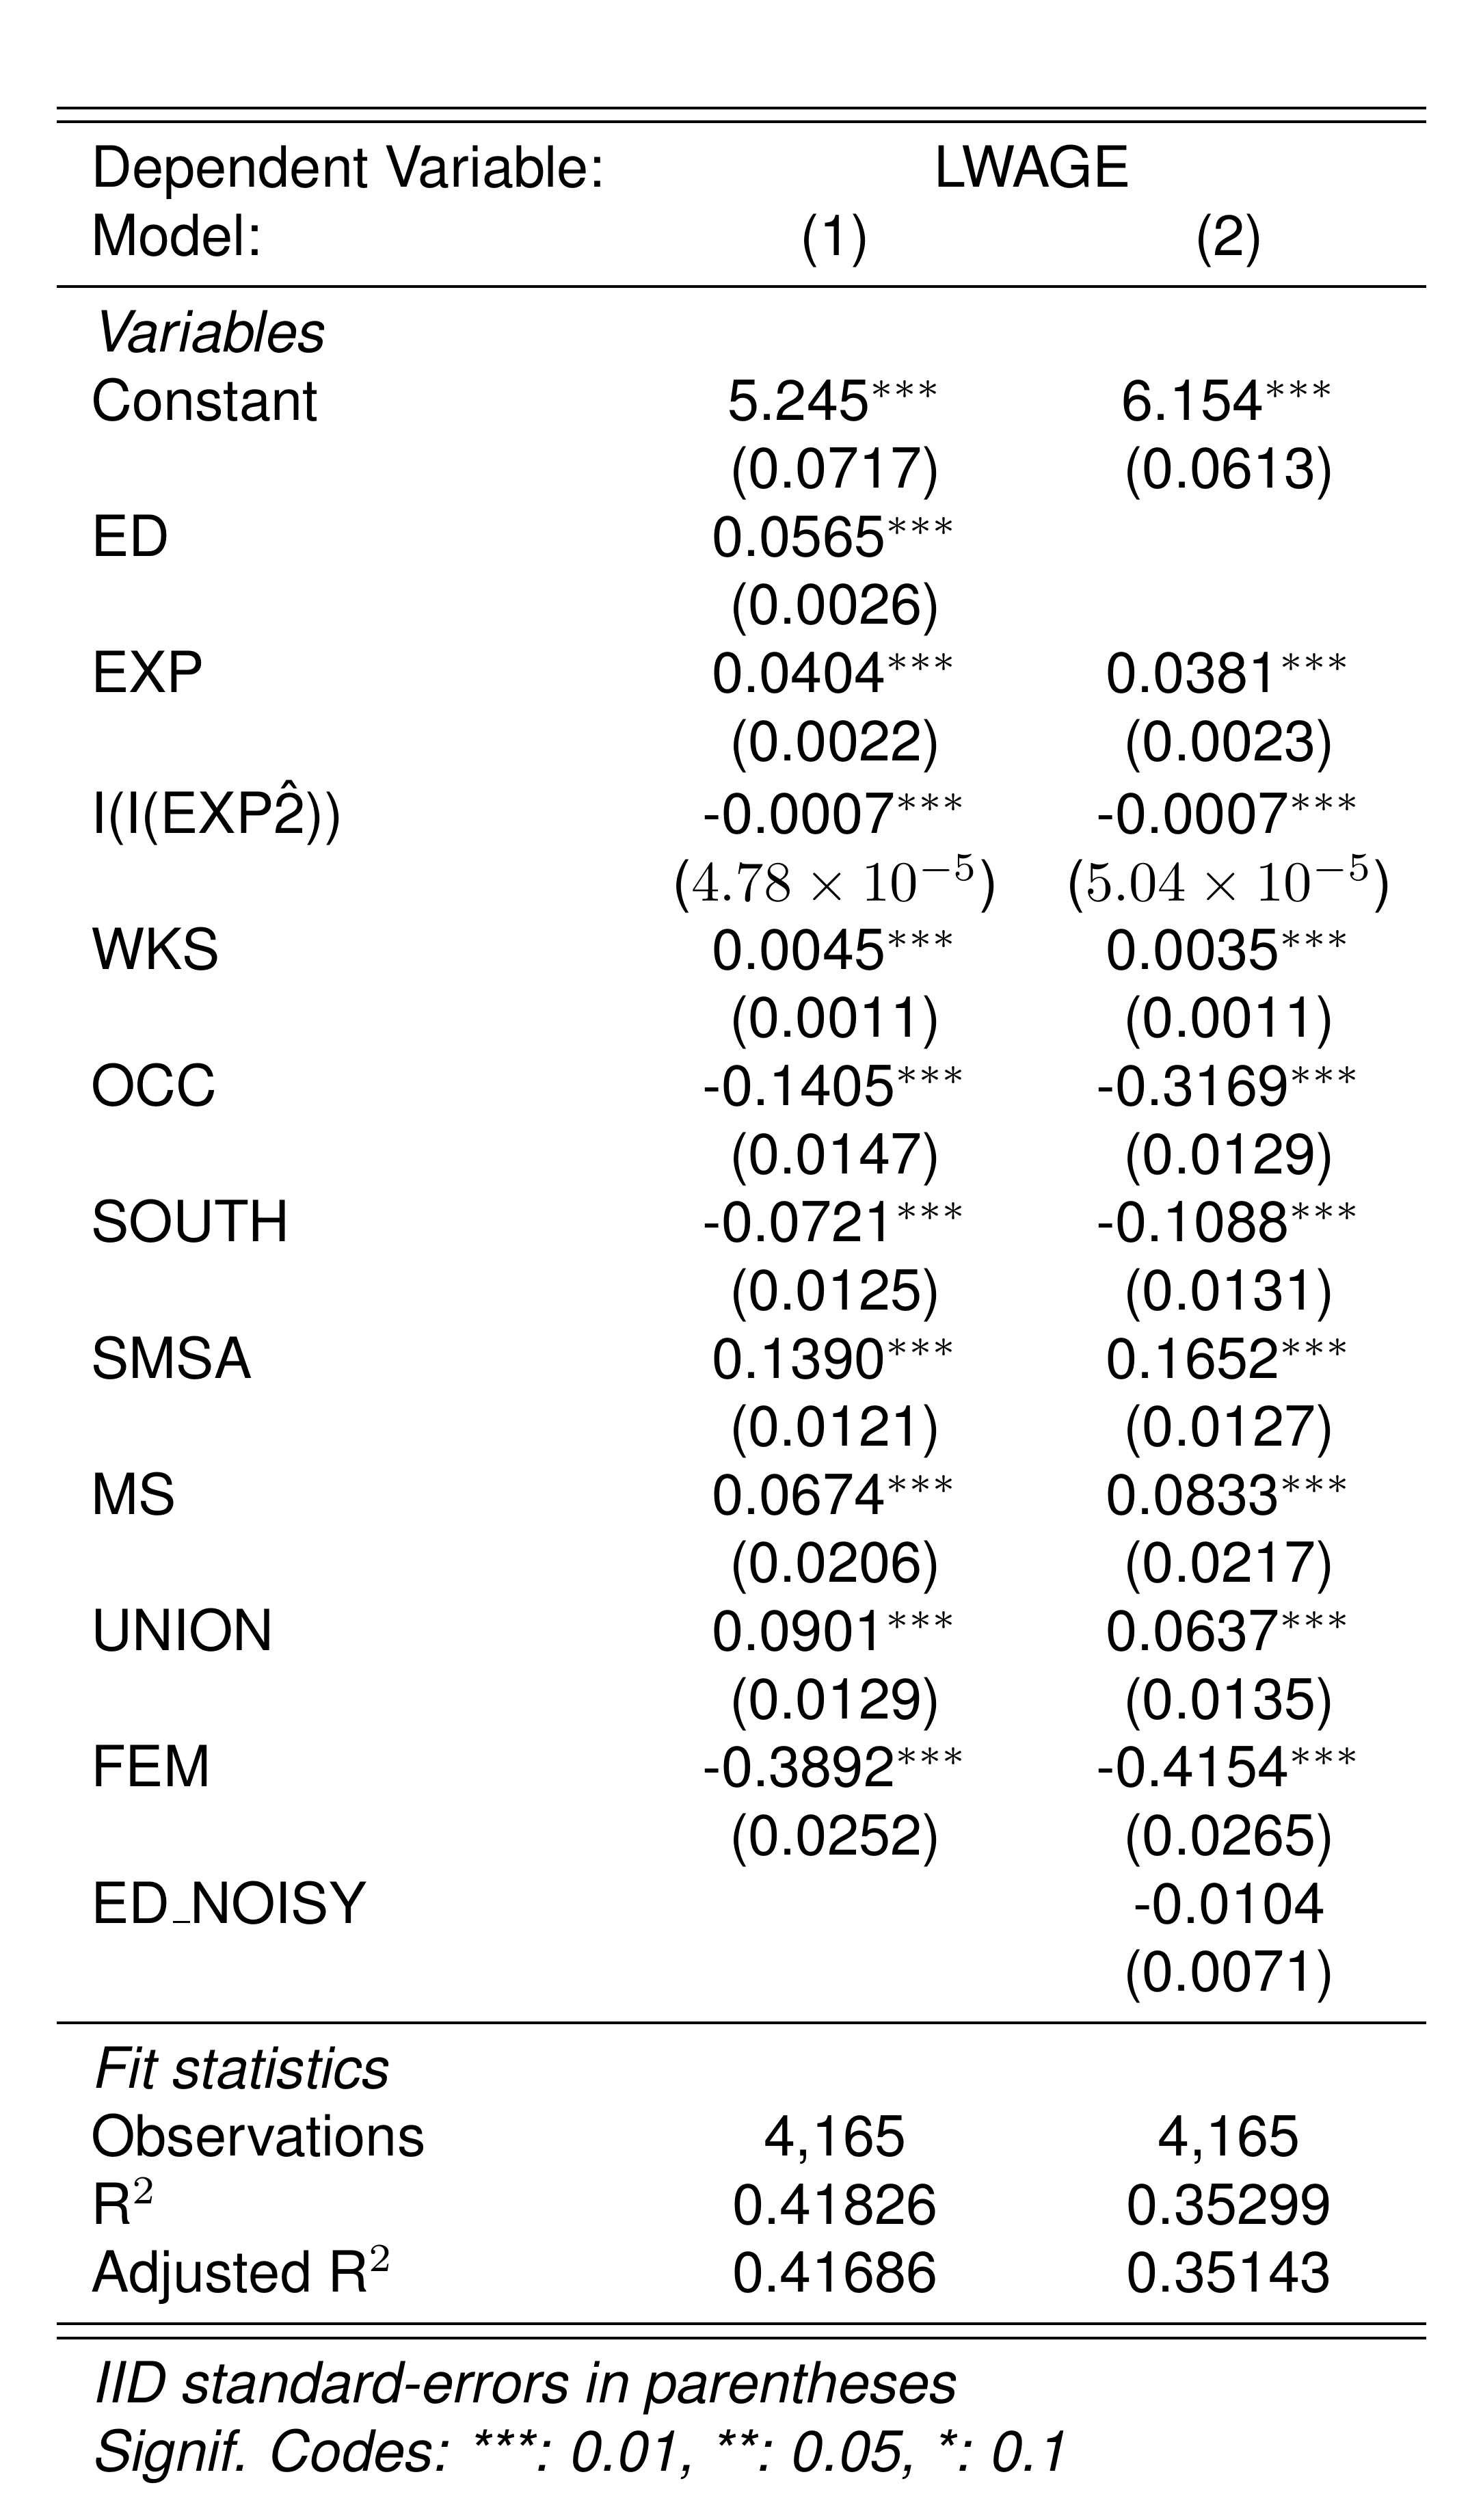
\includegraphics [width=.6\textwidth]	{table_noise}
\end{figure}
\end{column}
\end{columns}	
\end{frame}




% \begin{frame}[t]
% \frametitle{Heuristic Policies}

% \begin{columns}

% \column{0.5\textwidth}
% \begin{itemize}
% \item<1-> These are methods aiming to give a good but not necessarily optimal solution to a problem.
% \item<2-> There exist a number of such policies for bandit problems.
% \alt<1-9>{
% \item<3-9> Greedy policy:
% \begin{itemize}
% \normalsize
% \item<4-9> choose arm with greatest expected reward
% \item<5-9> ignores variability in prior distribution
% \item<6-9> quite good for Bernoulli bandits, but less effective for normal bandits
% \end{itemize}
% }{\only<10-14>{\item<10-> Next policy:
% \begin{itemize}
% \normalsize
% \item<11-14> comment 1
% \item<12-14> comment 2
% \item<13-14> comment 3\par
% \rule{0pt}{2.7cm}
% \end{itemize}}
% \only<15-18>{\item<15-> Another policy:
% \begin{itemize}
% \normalsize
% \item<16-18> Another comment 1
% \item<17-18> Another comment 2
% \item<18-18> Another comment 3\par
% \rule{0pt}{2.7cm}
% \end{itemize}}
% }
% \end{itemize}

% \column{0.3\textwidth}
% \vspace{-25pt}
% \uncover<7->{\begin{figure}
% \begin{center}
% \includegraphics[height = 2.7cm, trim=-1cm 0cm 0cm 0cm,clip=true,width=3cm]{example-image-a}
% \caption*{$(\alpha,\beta) = (1,1)$}
% \end{center}
% \end{figure}}
% \vspace{-25pt}
% \uncover<8->{
% \begin{figure}
% \begin{center}
% \includegraphics[height = 2.7cm, trim=-1cm 0cm 0cm 0cm,clip=true,width=3cm]{example-image-a}
% \caption*{$(\alpha,\beta) = (6,5)$}
% \end{center}
% \end{figure}}

% \column{0.2\textwidth} 
% \only<9>{$\Rightarrow$ play this arm} 
% \only<13-14>{$\Rightarrow$ play this arm with probability $\varepsilon$\vspace{80pt}} 
% \only<14>{$\Rightarrow$ play this arm with probability $1-\varepsilon$} 
% \end{columns} 
% \onslide<10>{\null}
% \end{frame}


\begin{frame}{Omitted Variables Bias, Revisited}
\begin{itemize}
	\item Suppose the econometrician only observes regressors ${\bf X} $, but the true model is\[
			{\bf y}= {\bf X} \boldsymbol{\beta} + {\bf z} \gamma + \boldsymbol{\varepsilon},
	\]

	\item The OLS estimator will equal\[
	{\bf b} = \left({\bf X}'{\bf X}\right)^{-1} {\bf X}' {\bf y} = \boldsymbol{\beta}  + \left({\bf X}'{\bf X}\right)^{-1} {\bf X}' {\bf z} \gamma + \left({\bf X}'{\bf X}\right)^{-1} {\bf X}' \boldsymbol{\varepsilon}
	\]

	\item The last term is mean zero given the strict exogeneity assumption.

	\item Note that the second term will not be zero if ${\bf X}$ and ${\bf z}$ are correlated;
	i.e. if $ {\bf X}' {\bf z} \ne 0$.

	\item Implication:  correlation between omitted variables and the observed regressors makes OLS biased.
\end{itemize}
\end{frame}

\begin{frame}{Omitted Variables Bias II}
\begin{itemize}
	\item Using the Frisch-Waugh theorem, we can show that \[
E\left[b_{OLS,k}|\boldsymbol{X},\boldsymbol{z}\right]=\beta_{k}+\gamma\left(\frac{Cov\left(z,x_{k}|\boldsymbol{X}_{-k}\right)}{Var\left(x_{k}|\boldsymbol{X}_{-k}\right)}\right)
\]
where $\boldsymbol{X}_{-k}$ refers to all the regressors besides $x_k$.

	\item Suppose positive correlation between regressor $x_k$ and omitted variable $z$.
	\item Also suppose $\beta_k>0$ and $\gamma>0$ so both variables have positive effects.
	\item Let's compare the average value of the dependent variable for $x_k=0$ and $x_k=1$. Two
	things change between these points:
\begin{itemize}
	\item Dependent variable $Y$ increases by $\beta_k$ because of direct effect of $x_k$.
	\item Value of $z$ should be higher because of the positive correlation between $x_k$ and $z$. 
	Higher values of $z$ also contribute to a higher dependent variable because $\gamma>0$. 
	\end{itemize}
\end{itemize}
\end{frame}


\begin{frame}{Omitted Variables Bias in Mincerian Regression}
\begin{columns}
\begin{column}{0.5\textwidth}
\begin{itemize}
	\item What sort of variables might the wage equation omit,
		and how would you expect them to affect the estimated
		coefficients?
\end{itemize}
\end{column}
\begin{column}{0.5\textwidth}
\begin{figure}
\flushleft
	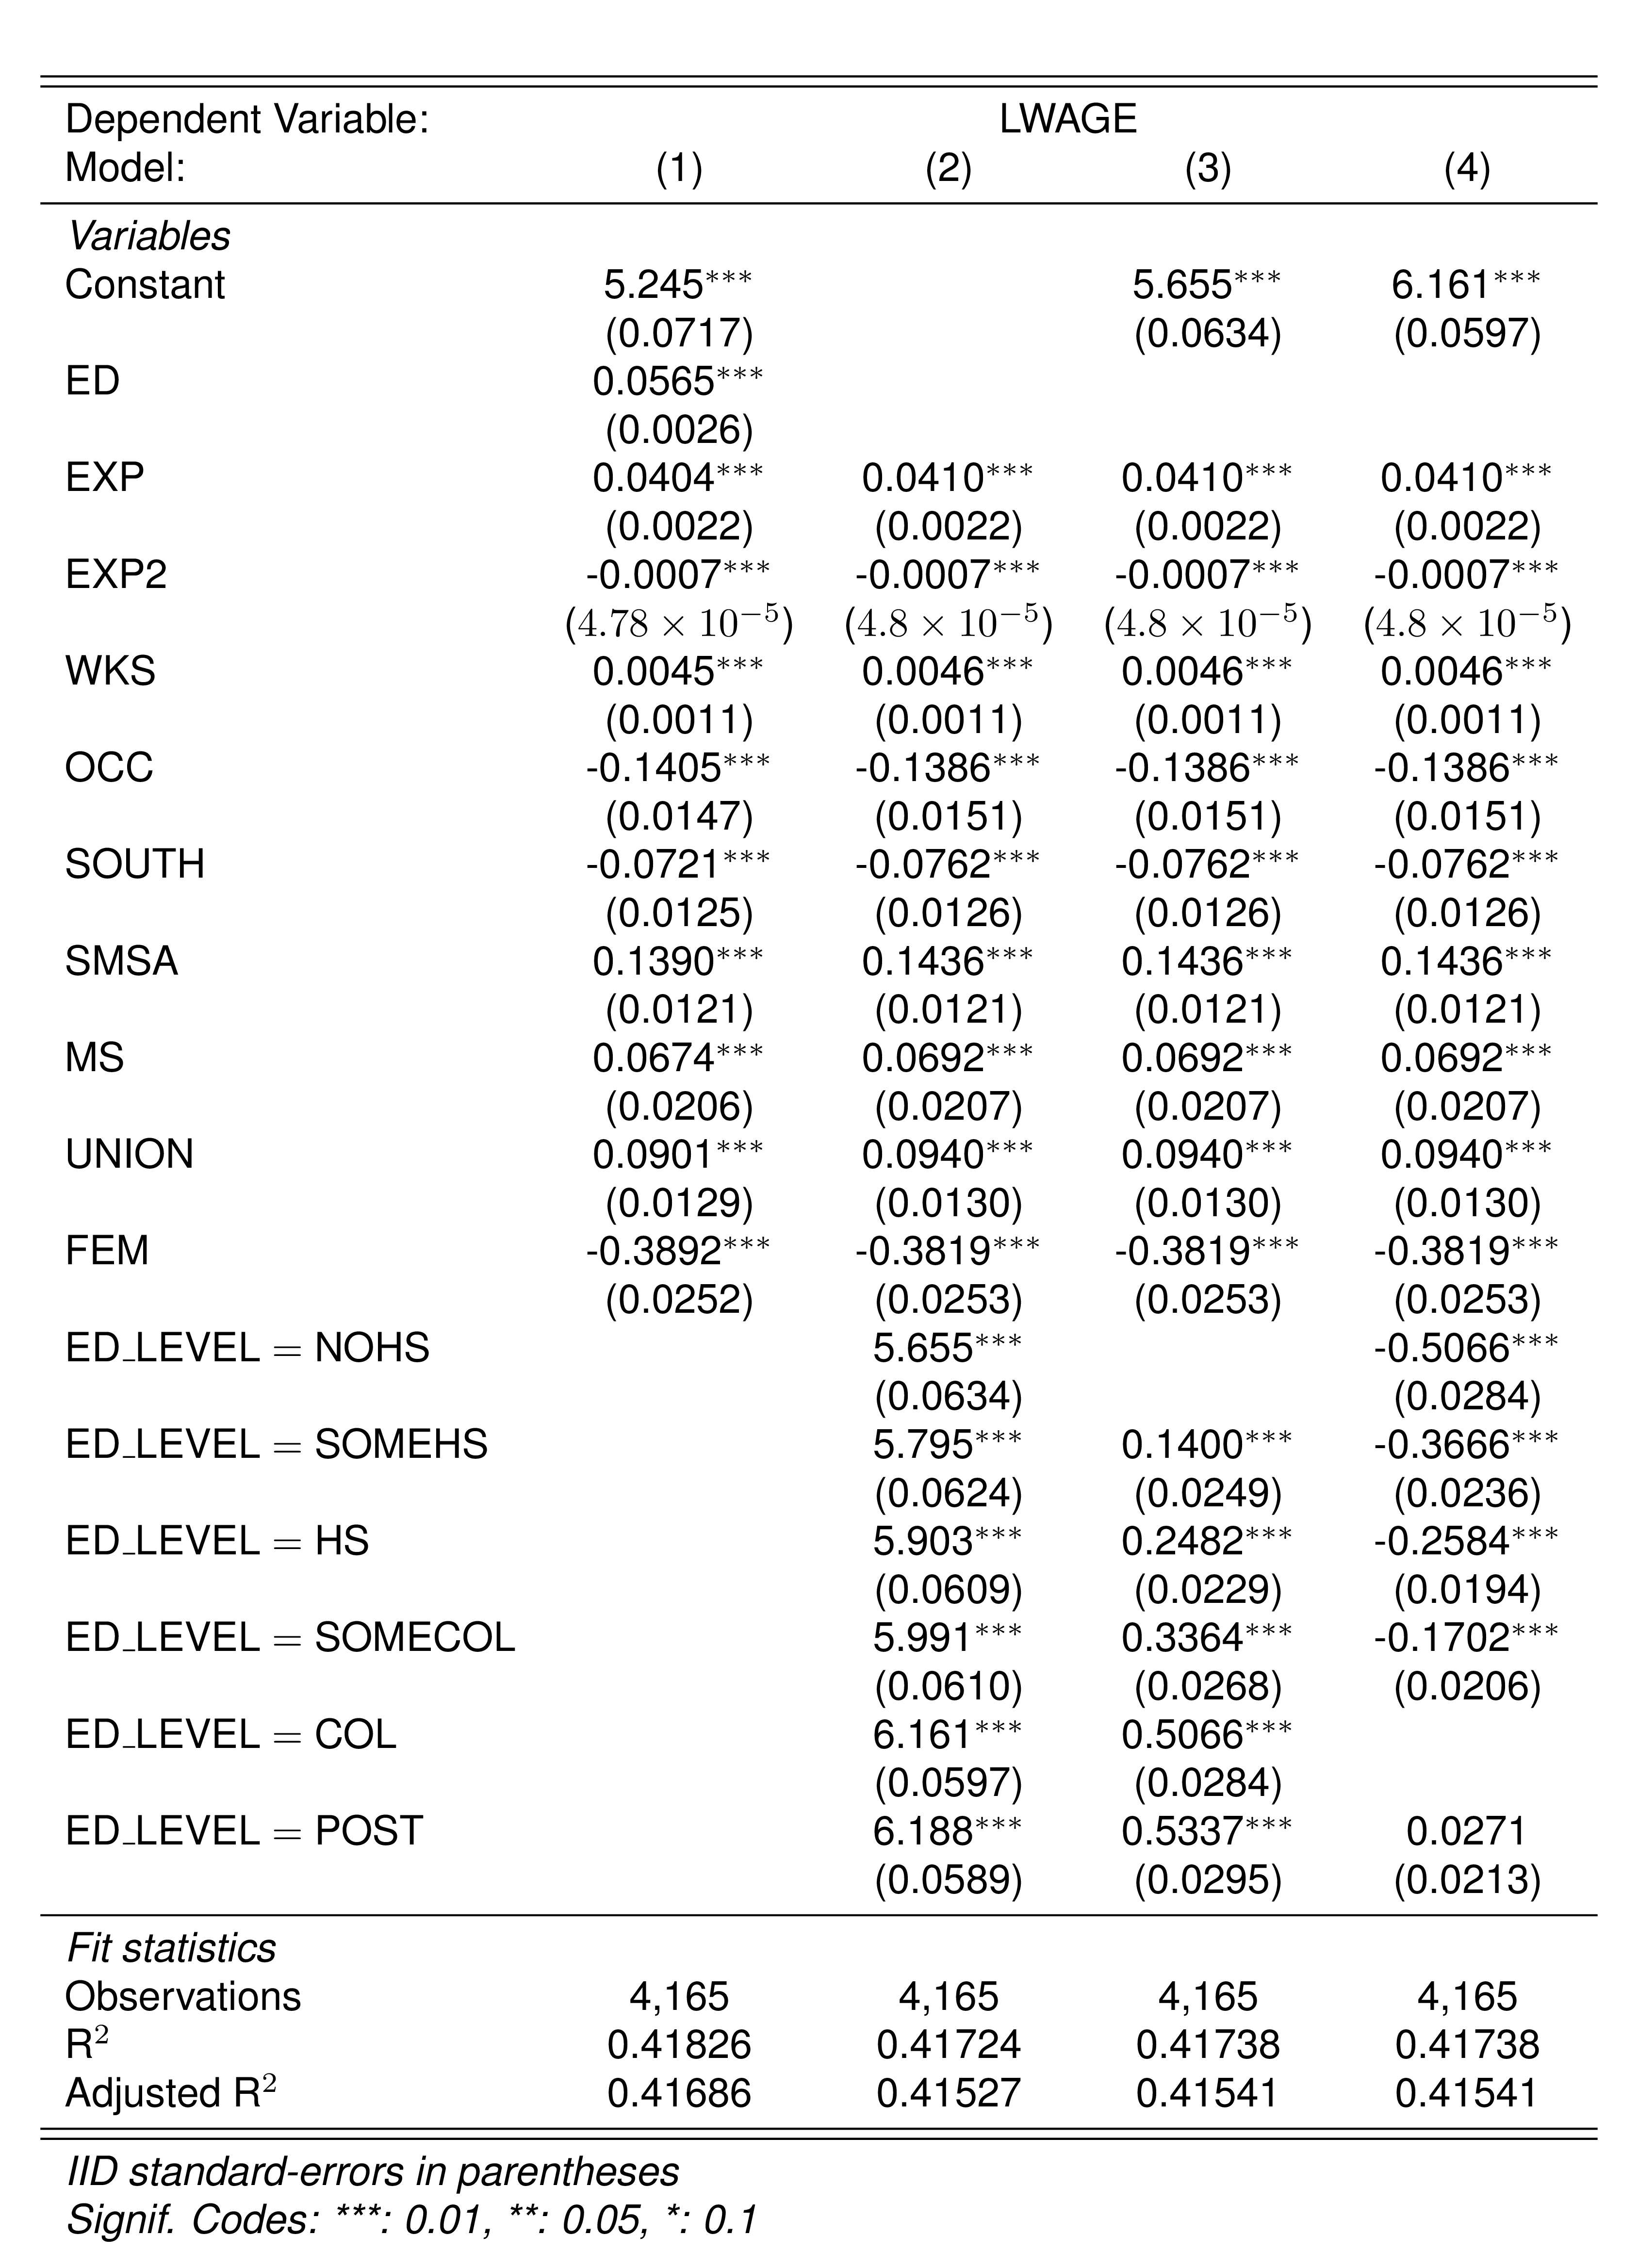
\includegraphics [width=.8\textwidth]	{table_1.png}
\end{figure}
\end{column}
\end{columns}	
\end{frame}

\end{document}